\section{Experimental setup}

In this work, we focus on the particular case of autonomous corridor navigation. 
For this purpose we use the vanishing point algorithm and PID control to maintain heading parallel to the corridor and stay in the middle of it. We implement our algorithm on a $1/10^{th}$ scale car we developed. This section covers the hardware, the algorithm, and the hardware level knobs which affect the performance of the closed loop system and energy consumption of the computation platform.

\subsection{The hardware}

For our experiments, we converted a Radio controlled Traxxas Rally car into an autonomous robot shown in Fig. \ref{fig:traxxas}, similar to the ones used in \cite{racecar_mit}.

The computation platform is a NVIDIA Jetson TK1. 
The Jetson has a quad-core ARM Cortex-A15 CPU and a NVIDIA Kepler GPU. 
This setup allows us to schedule tasks on the CPU or GPU while observing the effect of this on power consumption and timing of the algorithm. 
The Jetson runs Ubuntu for Tegra as the operating system, and the algorithms are implemented using ROS \cite{ros}. The control signals for the drive and steer motor on the platform are generated by a Teensy 3.1 microcontroller running a ROS node which converts the continuous output of the control software to a PWM signal that acts as an input to the motor controller on the Traxxas. 
Finally, the vanishing point algorithm implemented in OpenCV \cite{opencv} gets images from a front facing Point Grey Firefly MV camera capable of recording color images at upto a resolution of 752x480 pixels and upto a frame rate of 60 FPS. 

\subsection{Vanishing point-based corridor navigation}

The Vanishing point algorithm \cite{VP1} has been used extensively in indoor settings for navigating corridors autonomously \cite{VP2, VP3} and for outdoor lane detection \cite{gallagher2002ground}. 
The algorithm outputs the horizontal distance of the frame's vanishing point from the center of the frame. 
This distance is used by our car's controller to align the robot with the corridor. 
Figure \ref{fig:vp_viz} shows a visualization of Vanishing point operating on a frame collected from navigating in a corridor.


\begin{figure}[hbtp]
\centering
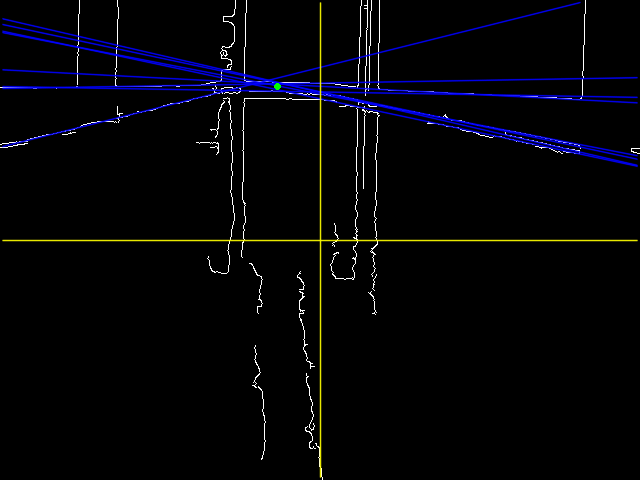
\includegraphics[scale=0.26]{Figs/image_176.png}
\caption{Visualization of the Vanishing point algorithm. The green dot shows the vanishing point.}
\label{fig:vp_viz} %diff freq same assignment}
\end{figure}



We focus on the major computational tasks that comprise the vanishing point algorithm, shown in Fig. \ref{fig:vanishing}.
They are:

\begin{itemize}
\item Blur: A Gaussian blur is applied on the image for de-noising.
\item Edge detection: We use the Canny Edge detector to find edges in the image.
\item Hough Transform: used to detect straight lines in the image.
\item RANSAC: used to select the parallel straight lines that best describe the sides of the corridor. These lines intersect in the image plane at the Vanishing Point.
\end{itemize}

\begin{figure}
	\centering
	\includegraphics[scale=0.3]{vanishing}
	\caption{The vanishing point algorithm with components running on either CPU or GPU at various frequencies, resulting in different power consumptions.}
	\label{fig:vanishing}		
\end{figure}
\subsection{Exploiting hardware level knobs}
With the vanishing point algorithm, we can execute the Blur, the Edge detection and the Hough transform on either the CPU or the GPU. 
RANSAC runs fast enough to not have a significant impact on the total execution time, so we do not consider running it on the GPU.
Execution on the GPU results, in general, in a speed-up over the CPU but at the cost of higher power draw from the Jetson. 
Additionally, on the Jetson, we can control the performance of the CPU and GPU by changing the clock frequencies at which they operate. 
This gives us multi-dimensional knobs on the hardware level that we can control to trade-off computation speed and power consumption.




